\documentclass[10pt]{article}
\usepackage[margin=0.8in]{geometry}
\usepackage{graphicx}
\begin{document}
\begin{center}
{\Large N53 K220 first run attempt: timing-wrapper failure}\par
2026-10-12 17:35 UTC; run 20261012T1735Z
\end{center}
\noindent The frozen source, public targets, seeds and schedule in
\texttt{../../FROZEN.json} were used inside the filesystem sandbox.
Eight child outputs were emitted. macOS \texttt{/usr/bin/time -l} then
returned code 1 and reported \texttt{sysctl kern.clockrate: Operation
not permitted}; it supplied no maximum resident set size. Each of the
eight statuses is \texttt{INCOMPLETE}; the ninth cell was interrupted
without status when the run stopped.

\medskip
\noindent This is an infrastructure failure of the measurement wrapper.
The eight cells are excluded from timing comparison. Their raw intents,
outputs, stderr and statuses are retained at
\texttt{../../runs\_sandbox\_wrapper\_failure\_20261012T1735Z/}.
A direct wrapper check outside the sandbox returned code 0 with maximum
RSS; the identical frozen binaries and inputs then ran in the
20261012T1737Z series.

\medskip
\begin{center}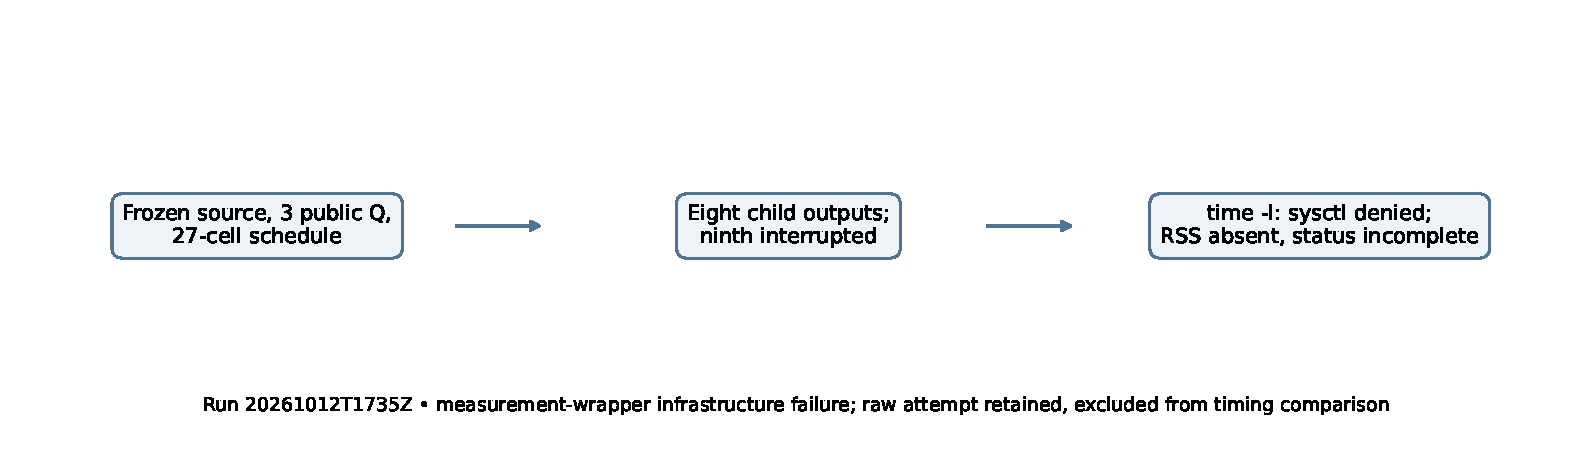
\includegraphics[width=\linewidth]{failure_path.pdf}\end{center}
\end{document}
